\section{Introduction}

In this chapter, we introduce the vision of what constitutes a Cognitive and
Immersive System, followed with a real-world implementation of various
components. As discussed in Chapter~\ref{chap:introduction}, we expect that
while a CAIS may be deployed into a variety of environments of differing
capabilities, they will all follow the same overarching definition and function.
For any given system, it is composed of three areas, that operate in a
cyclical flow, where sensors feed decision processes that feed output mechanisms.
However, at the core of this is that these systems are not just merely ``intelligent''
like prior art, where the room is able to answer queries about some problem domain,
but rather that it is ``cognitively intelligent'', where the system can reason
and answer questions about the cognitive states of agents and their cognitive
states towards the domain.

%%%%%%%%%%%%%%%%%%%%%%%%%%%%%%%%%%%%%%%%%%%%%%%%%%%%%%%%%%%%%%%%%%%%%%
\begin{figure}
    \centering
    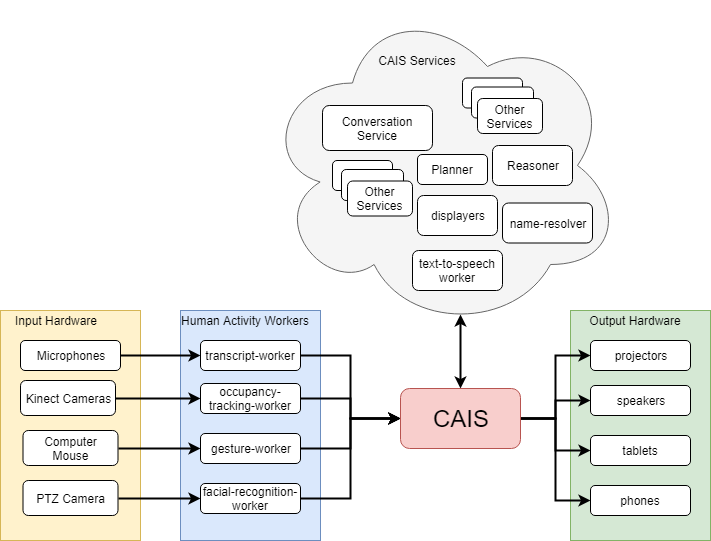
\includegraphics[width=0.5\columnwidth]{chapters/02_technology/figures/cais_high_level.png}
    \caption{High level diagram of CAIS architecture.}
    \label{fig:cycle-cais}
\end{figure}
%%%%%%%%%%%%%%%%%%%%%%%%%%%%%%%%%%%%%%%%%%%%%%%%%%%%%%%%%%%%%%%%%%%%%%
